\documentclass[a4paper, 11pt]{exam}
\usepackage{titling}
\newcommand{\subtitle}[1]{%
  \posttitle{%
    \par\end{center}
    \begin{center}\large#1\end{center}
    }%
}

\usepackage{url}
\usepackage{amsmath,amsthm,enumitem,amssymb}
\usepackage{algorithm,algorithmic,amsmath}
\usepackage{graphicx}
\usepackage{hyperref}
\renewcommand{\labelenumii}{\roman{enumii}}
\usepackage{courier}
\usepackage{epsfig}

\title{Homework Assignment 4}
\subtitle{CS/ECE 6810: Computer Architecture \\
Nov 28, 2018\\
Jake Pitkin, u0891770}

\author{ \\
\textbf{Memory Systems}}
\date{Due Date: December 11, 2018.\\
(120 points)}

\begin{document}
\maketitle

\begin{enumerate}

\item \textbf {Virtually Indexed Cache.}
Referring to the lecture slide on virtual address translation and TLB, explain the
challenges if the number of bits in the page offset does not equal the number of
bits in the sum of ``Index'' and ``Byte'' (Please see \url{http://www.cs.utah.edu/~bojnordi/classes/6810/f18/slides/18-tlb.pdf}). 
You are asked to identify the issues and their corresponding solutions from the literature.
\textbf{(20 points)}

\textbf { Special Instructions :}
\begin{enumerate}
	\item Strictly NO collaboration or brainstorming on this question is accepted.
	\item Mention ALL references used to answer this question.
	If no references are mentioned, 0 points will be awarded.
\end{enumerate}



\item \textbf {Virtual Memory and TLB.}
Consider an operating system (OS) using 1KB pages for mapping virtual to physical addresses.
Initially, the TLB is empty and all of the required pages for the user application as well as the page table are stored in the main memory.
(There is no need to transfer data between main memory and the storage unit.)
Every access to the TLB and main memory takes respectively 1 and 200 processor cycles.
The TLB can store up 16 entries.

\begin{enumerate}
	\item Assuming that the main memory size is 1MB and the page table has 2048 entries, show the number of required bits for the physical and virtual address fields. \textbf{(5 points)}
	
	Given 1KB pages, both the physical and virtual address fields will require 10 offset bits. The page table has 2048 entries which will require 11 bits to address. Main memory is 1MB with 1KB pages, so it contains 1024 pages which will require 10 bits to address.
	
	\fbox{Virtual address = Virtual Page No + offset = 11 + 10 = 21 bits}
	
	\fbox{Physical address = Page frame No + offset = 10 + 10 = 20 bits}
	\item Assume that the user application only generates five memory requests to the virtual addresses \texttt{0000}, \texttt{0004}, \texttt{0008}, \texttt{0800}, and \texttt{0804} (all in hexadecimal);
	the first request is ready at time 0; and
	the processor generates every next request immediately after serving the current one.
	Please find the execution time with and without using TLB in the proposed system and compute the attainable speedup due to using TLB.
	\textbf{(15 points)}
\end{enumerate}






\item \textbf {DRAM Address Mapping.}
Consider a simple in-order DRAM command scheduler.
Initially, all DRAM banks are precharged and the scheduling queue contains seven read requests to the following physical addresses: 
\texttt{00040108},
\texttt{01040101},
\texttt{FF042864},
\texttt{A5181234},
\texttt{A5184321},
\texttt{00161804}, and
\texttt{01040104}
(all in hexadecimal).
Using the following address mapping scheme, show all the required commands issued by the controller to serve the memory requests.
\textbf{(20 points)}

\begin{center}
	\begin{tabular}{|c|c|c|c|c|}
		\hline
		row (10)&bank (4)&rank (2)&channel (0)&column (16) \\
		\hline
	\end{tabular}
\end{center}

\item \textbf{DRAM Row (Page) Management.}
A computer system includes DRAM and CPU.
The DRAM subsystem comprises a single channel/rank/bank.
CPU generates a sequence of memory requests to rows \texttt{X} and \texttt{Y}.
Table below shows the accessed rows by the memory requests and their arrival times at the DRAM controller.
Assume that the DRAM bank is precharged initially; the DRAM scheduling queue has infinite size; and the memory interface must enforce the following timing constraints (all in $ns$):
tCAS = 3, tRAS = 20, tRP = 20, tRCD = 10, and tBURST = 4. 

\begin{center}
	\begin{tabular}{|c|c|}
		\hline
		\textbf{Accessed Row} & \textbf{Arrival time ($ns$)} \\
		\hline
		\texttt{X}  & 10 \\
		\hline
		\texttt{X}  & 70 \\
		\hline
		\texttt{Y}  & 80 \\
		\hline
		\texttt{X}  & 85 \\
		\hline
		\texttt{Y}  & 110 \\
		\hline
		\texttt{X} & 210 \\
		\hline
	\end{tabular}
\end{center}

The goal is to evaluate two row management policies, namely \textit{open-page} and \textit{closed-page}.
Show all the necessary transactions on the command, address, and data buses for each policies.
Discuss which policy performs better for the given example.
(Note: you are allowed to reorder requests already waiting in the memory controller.)
\textbf{(20 points)}
\begin{figure}[h!]
	\begin{center}
		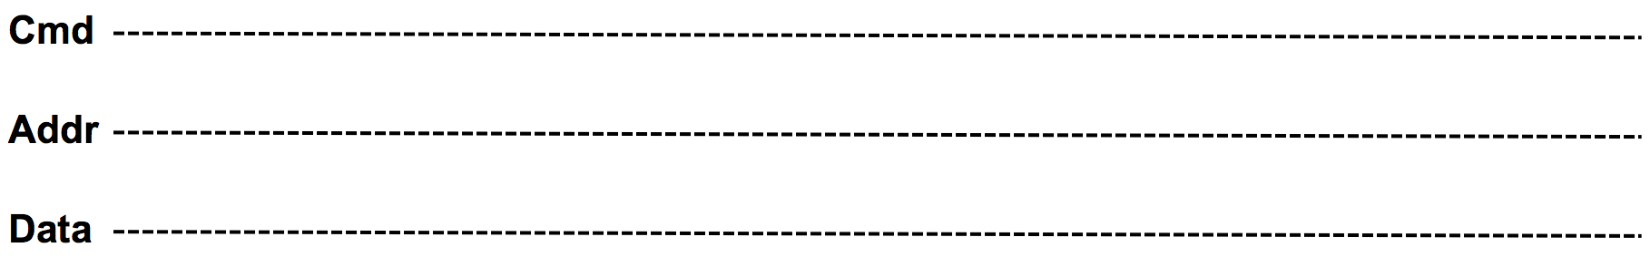
\epsfig{file=timing.pdf, width = \columnwidth}
	\end{center}
\end{figure}

\item \textbf{Data TLB.}
Consider the following  pseudo code, in which \textbf{X} and \textbf{Y} are allocated as contiguous integer arrays in memory and are aligned to the 4KB boundaries.
Assume that \textbf{k} and \textbf{l} are allocated in the register file with no need for memory accesses.
We execute the code on a machine with virtual memory where the integer type (\textbf{int}) is 4 bytes wide.
Assume that the system include a direct-mapped D-TLB with 1024 entries for serving all data accesses only.
Initially, the D-TLB is empty.
Find the hit rate of the D-TLB when running the code.
\textbf{(20 points)}
\begin{algorithm}
	\textbf{\#define M 1024} \\
	\textbf{int X[M*M];} \\
	\textbf{int Y[M*M];} \\
	\textbf{int k, l;}
	\begin{algorithmic}	
		\FOR{$(k = 0; k < M; k++)$}
		\FOR{$(l = 0; l < M; l++)$}
		\STATE \texttt{Y[l*M+k] = X[k*M+l];}
		\ENDFOR
		\ENDFOR
	\end{algorithmic}
\end{algorithm}


\end{enumerate}
\end{document}
